\documentclass{article}
\usepackage[utf8]{inputenc}
\usepackage{graphicx} % Required for including images
\usepackage{amsmath, amssymb} % Required for math features
\usepackage{hyperref} % For hyperlinks
\usepackage{natbib} % For bibliography
\usepackage{geometry} % For page dimensions and margins
\geometry{a4paper, margin=1.2in}

\title{Machine Learning Project Report: Neural Network Implementation on MNIST Dataset}
\author{Noé Bourgeois}
\date{Academic Year 2023-2024}

\begin{document}

\maketitle

\begin{abstract}
% Write your abstract here
\end{abstract}

\section{Introduction}
% Introduce the project, its objectives, and significance

% \section{Methodology}
\section{Experimentation Framework}
% Describe the methodology, including neural network architecture, 
% forward propagation, error calculation, and backpropagation

\subsection{Neural Network Architecture}
% Details about the neural network layers, activation functions, etc.

\subsection{Forward Propagation}
% Explain the forward propagation process

\subsection{Error Calculation}
% Describe how the error is calculated (mean squared error, etc.)

\subsection{Backpropagation}
% Explain the backpropagation process for weight updates


\section{Results}
% Present the results of your experiments
% Include graphs, tables, and confusion matrix visualizations
\subsection{Training}
\subsection{Testing}
\subsubsection{Confusion Matrix}
% graph:
\begin{figure}
    \centering
    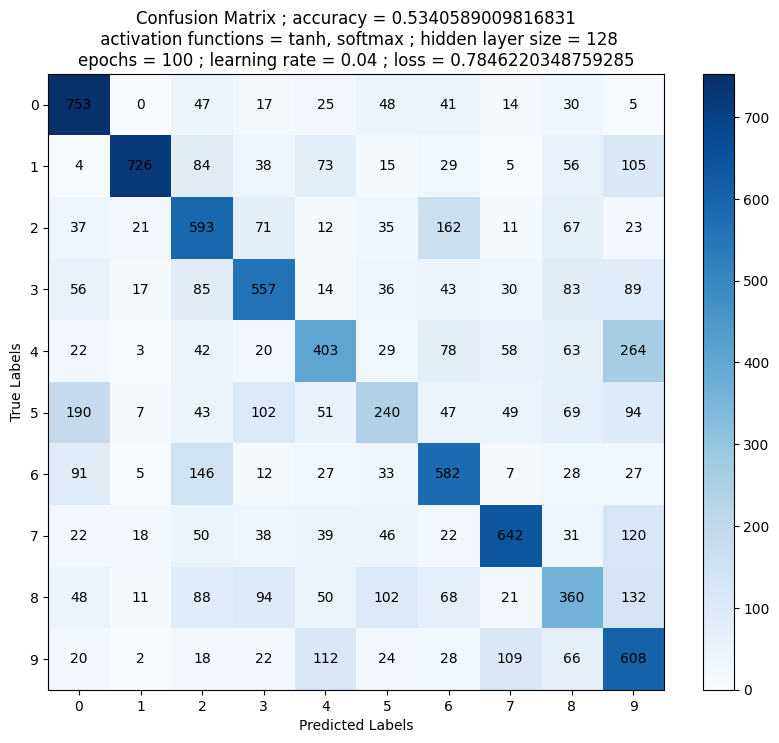
\includegraphics[width=\textwidth]{media/confusion/confusion_matrix_activation_functions_tanh_softmax_hidden_layer_size_128_epochs_100_learning_rate_0.04_loss_0.7846220348759285.png}
    \caption{Confusion Matrix for tanh activation function, softmax output function, 1 hidden layer of 128 neurons, 100 epochs, 0.04 learning rate, and 0.7846220348759285 loss.}
    \label{fig:confusion}
\end{figure}
\subsubsection{Accuracy}
\subsubsection{Prediction}
\begin{figure}
    \centering
    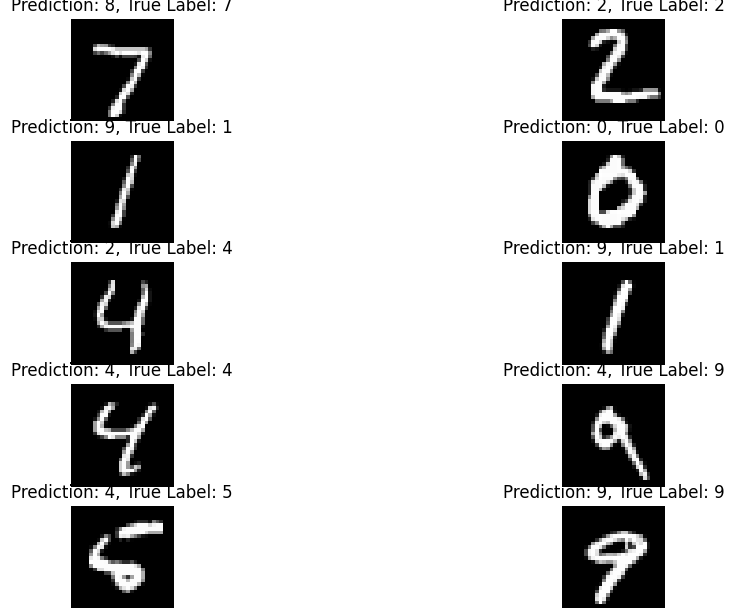
\includegraphics[width=\textwidth]{media/prediction/4.png}
    \caption{Prediction}
    \label{fig:Prediction}
\end{figure}
\subsection{Convolution}
98.8\% accuracy
\subsubsection{Feature Learning}
Unlike traditional machine learning algorithms,
CNNs automatically detect important features without
 any human intervention. 
 This is achieved through the use of filters to the input, 
 enabling the model to learn features directly 
 from the images.

\subsubsection{Spatial Hierarchy of Features}
CNNs are adept at understanding the spatial hierarchy 
in images. 
Early layers might detect simple features like edges or corners,
 while deeper layers can recognize more complex features 
 like shapes or specific objects. 
This hierarchical approach is particularly effective for
image classification.

\subsubsection{Parameter Sharing and Local Connectivity}
In CNNs, the same weights (filters) are shared across
different parts of an image. 
This not only reduces the number of parameters the network
needs to learn, making the model more efficient, 
but also allows the network to recognize features
regardless of their position in the input image.

\subsubsection{Robustness to Image Variations}
CNNs are less sensitive to variations and distortions 
in images, such as slight shifts, rotations, 
and changes in scale. 
This robustness is due to the pooling layers commonly used
in CNNs, which help in making the detection of features
invariant to small changes in the position of the feature
in the image.

\subsubsection{Efficient Handling of High-Dimensional Data}
Images are high-dimensional data 
(considering each pixel as a dimension). 
CNNs can manage this high dimensionality better 
than many traditional algorithms, 
which often struggle with the curse of dimensionality.

\subsubsection{Specialization for Image Data}
The convolutional layers are particularly well-suited 
for processing images pixels that are spatially close 
to each other, capturing local dependencies effectively.
This specialization perfectly matches the structure of 
characters, in our case digits, images.

\subsubsection{Confusion Matrix}
% graph:
\begin{figure}
    \centering
    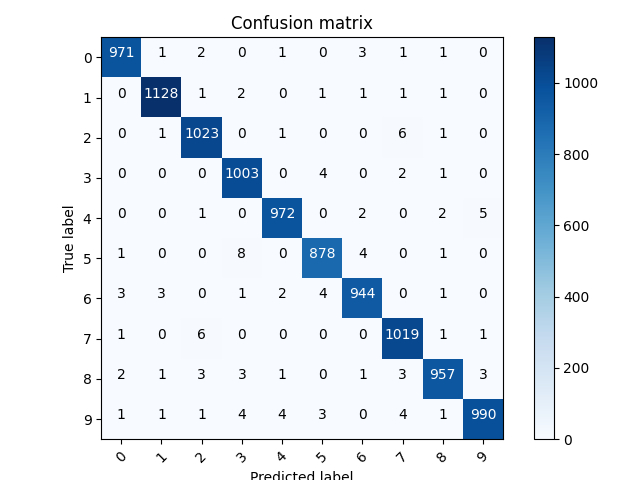
\includegraphics[width=\textwidth]{media/convolution/Figure_1.png}
    \caption{Confusion Matrix for convolutional model.}
    \label{fig:convolution_confusion}
\end{figure}

\section{Analysis}
% Discuss the results, what they mean, and any conclusions you can draw
The results indicate a strong dependency of 
neural network performance on its 
architecture and 
hyperparameters. 
\subsection{Hidden Layer Size impact}
biggest impact
\subsection{Learning Rate impact}
reducing learning rate increases accuracy
\subsection{Epochs impact}
augmenting epochs is good only if neurons quantity and learning rate decay are augmented exponentially.
Otherwise, overfitting occurs.

\subsection{Convolutional Model}
The convolutional model particularly excelled in 
image classification tasks.
\section{Conclusion}
% Summarize the main findings and future work
\subsection{Main Findings}
The study demonstrates the effectiveness of 
neural networks in digit classification. 
\subsection{Tools}
\subsubsection{Assistance}
\begin{itemize}
    \item ChatGPT
\end{itemize}
\subsection{Future Work}
We will continue exploring 
deeper and evolving architectures and 
implementing advanced techniques like 
dropout and batch normalization at different intensities
at particular network states.


\section{References}
% Include your references here
\bibliographystyle{plain}
\bibliography{references} % references.bib should be the name of your BibTeX file

\end{document}
